
\PassOptionsToPackage{numbers,sort&compress}{natbib}
\documentclass{article}
\usepackage[preprint]{neurips_2025}
\usepackage[utf8]{inputenc}
\usepackage[T1]{fontenc}
\usepackage{hyperref}
\usepackage{url}
\usepackage{xurl}
\usepackage{booktabs}
\usepackage{amsmath,amssymb,amsfonts}
\usepackage{nicefrac}
\usepackage{microtype}
\usepackage{xcolor}
\usepackage{graphicx}
\usepackage{tabularx}
\usepackage{threeparttable}
\usepackage{subcaption}
\usepackage{multirow}
\usepackage{makecell}
\usepackage{enumitem}
\usepackage{siunitx}
\usepackage{cleveref}
\hypersetup{
  hidelinks,
  pdftitle={Same-Size Capability Transfer Reveals a Performance--Localization Tradeoff in Deterministic Function Calling},
  pdfauthor={Ali Uyar}
}
\usepackage{float}
\sisetup{detect-all=true, table-number-alignment=center, group-separator={,}, group-digits=integer, output-decimal-marker={.}, group-minimum-digits=4}
\setlist[itemize]{leftmargin=*, topsep=1pt, itemsep=1pt}
\setlength{\abovecaptionskip}{4pt}
\setlength{\belowcaptionskip}{-2pt}
\title{Same-Size Capability Transfer Reveals a Performance--Localization Tradeoff in Deterministic Function Calling}
\author{Ali Uyar\\Independent Researcher}

\begin{document}
\maketitle

\begin{abstract}
We study whether task-specific function-calling behavior can be transplanted from a donor back into an untuned same-size base model using fixed modules instead of full retraining. Our setting is intentionally narrow and fully deterministic: within-family Gemma models, single-turn function calling, frozen manifests, exact JSON grading, and a primary metric defined on SchemaShift and NoCall stress slices. The donor substantially outperforms the base on the primary strict metric, from $0.0375$ to $0.1781$ (delta $0.1406$, 95\% CI [$0.1208$, $0.1604$]). A sparse same-size intervention selected by a locked discovery pipeline reaches $0.2068$ strict success on the discovery seed and $0.1658$ mean strict success across three seeds, while a matched dense shortcut reaches $0.2177$ mean strict success across the same seeds. Sparse structure is nevertheless non-random: a locked one-feature subset retains $47.1\%$ of the full sparse gain and beats random one-feature controls, and one-vector steering is clearly weaker at $0.1078$ strict success. The resulting picture is therefore not sparse superiority. Instead, we find a real performance--localization tradeoff: same-size transfer is real in this setting, dense parameter-matched modules recover more raw task performance, and sparse modules provide partial localization signal. We present this deterministic function-calling setup as a concrete testbed for studying constructive capability transfer under tight claim discipline.
\end{abstract}

\section{Introduction}
Our question is constructive rather than descriptive: can we move a narrow capability from a trained donor into an untuned model without simply retraining the target again? That question matters for post-training science, mechanistic interpretability, and model editing. If a capability can be transferred through a small fixed module, we learn not only that the capability is movable, but also something about how concentrated or diffuse the relevant computation is.

We study that question in a deliberately narrow regime: same-size, within-family capability transfer for single-turn function calling. Function calling is a useful setting because it admits deterministic grading and naturally separates several failure modes: whether to call a tool or abstain, which tool to choose, and whether arguments are grounded correctly. Recent benchmarks such as BFCL argue that deterministic tool-use evaluation is essential for measuring this kind of behavior reliably \citep{patil2025bfcl}. We adopt that spirit, but instead of building a broad benchmark, we freeze a compact testbed derived from Mobile Actions \citep{google2025mobileactions} and use it to ask a mechanistic transfer question.

The resulting picture is not one of sparse superiority. The evidence supports a more interesting thesis. Same-size transfer is real on this task: the sparse intervention is not noise, steering is clearly weaker, and pruning plus random-subset controls reveal real localization structure. But when we compare matched multiseed performance under effectively identical parameter budgets, a dense module outperforms the sparse one. This exposes a performance--localization tradeoff rather than a single dominant mechanism.

Our main contributions are:
\begin{itemize}
  \item a locked same-size transfer testbed for deterministic single-turn function calling with frozen manifests, exact grading, and explicit schema-shift and NoCall stress slices;
  \item evidence that same-size transfer is real in this setting, with a donor gap of $0.1406$ on the primary metric and positive sparse transfer across three seeds;
  \item evidence that raw transfer performance and mechanistic compactness separate: dense parameter-matched modules win the final multiseed comparison, while sparse modules retain partial localization signal through pruning and control analyses.
\end{itemize}

The scope is intentionally limited. We do not claim cross-scale transfer, recipient data efficiency, universal model editing, uniquely identified sparse circuits, or clean schema-shift semantic transfer. The contribution is narrower and, we think, cleaner: a well-measured same-size transfer result that reveals a real tradeoff.

\section{Related framing and positioning}
This work sits at the intersection of deterministic function-calling evaluation and mechanistic model diffing. On the evaluation side, BFCL established that tool-use assessment benefits from exact, programmatic scoring rather than free-form judging \citep{patil2025bfcl}. Google released Mobile Actions and FunctionGemma as a compact on-device function-calling stack \citep{google2025mobileactions}. We use that ecosystem as a source of structured supervision, but our goal is not a new leaderboard score. Our goal is a controlled transfer setting.

On the mechanistic side, recent work has shown that learned mappings can transfer representations, probes, and steering vectors across models \citep{chen2025stitching, oozeer2025activationtransfer}. Model-diffing methods based on transcoders and crosscoders study how fine-tuning changes internal computation and how much of that computation can be approximated by learned sparse modules \citep{paulo2025transcoders, hu2026transcoderadapters, kassem2026deltacrosscoder}. Gemma Scope 2 makes this family of analysis practical on Gemma by releasing open SAEs and transcoders across the model family \citep{google2025gemmascope, deepmind2025gemmascopeblog}.

We differ from that prior work in three ways. First, we focus on \emph{same-size} transfer, not cross-scale transfer. Second, we make the setting deterministic and claim-audited: frozen manifests, frozen control suite, no LLM judge, and explicit claim weakening when evidence fails. Third, we compare sparse, dense, and steering interventions at the same hook site under matched or near-matched parameter budgets. The outcome is therefore not just ``can a sparse module do something?'' but ``what does sparse buy relative to dense and steering in a fixed transfer setting?''

\section{Locked setting and method}
\subsection{Task and primary metric}
We use a within-family same-size setting with an untuned source base model $B$ and a task-trained donor $D$ of the same size. In the locked \texttt{V24} path, both are Gemma-family 1B instruction-tuned models. Each example provides a user request, an inventory of tool schemas, and a canonical JSON target of the form
\begin{equation}
\{\texttt{"name"}: \tau,\; \texttt{"arguments"}: a\}
\end{equation}
where $\tau$ is either a tool name or \texttt{NO\_TOOL}. The assistant target is always exactly one JSON object and no prose.

Evaluation is deterministic. The \emph{strict} metric requires a single valid JSON object with the correct tool choice or abstention decision and correct normalized arguments. The \emph{semantic} metric parses the first valid JSON object and scores the normalized content even if trailing text exists. Our primary metric is strict full-call success on the union of three frozen stress slices: \textsc{SchemaShift}, \textsc{NoCall-MissingTool}, and \textsc{NoCall-Unsupported}. This primary set contains 1,920 examples: 640 per slice.

\subsection{Discovery and confirmation protocol}
We follow a locked two-stage protocol. A discovery seed is used to scan four candidate MLP layers and a fixed gain grid under frozen manifests. The selected sparse configuration is then re-evaluated on the frozen manifests and compared to dense and steering controls built at the same site. Finally, sparse and dense are rerun across three seeds (17, 29, and 43) for the confirmatory comparison. The goal is to avoid a one-off cherry-picked checkpoint.

Before any transplant work, we require a donor-gap gate on the primary metric. That gate passes: the base reaches $0.0375$, the donor reaches $0.178125$, and the donor-base delta is $0.140625$ with bootstrap 95\% CI [$0.120833$, $0.160430$].

\subsection{Sparse transplant and matched controls}
At a selected MLP site $l$, let $x_l$ be the MLP input and let $u_l^B$ and $u_l^D$ denote the MLP outputs of the base and donor under teacher forcing on matched examples. We fit a module to approximate the donor-minus-base delta,
\begin{equation}
\Delta_l(x_l) = u_l^D - u_l^B.
\end{equation}
The sparse module uses a TopK bottleneck,
\begin{align}
 z &= \operatorname{TopK}(\operatorname{SiLU}(W_{\mathrm{enc}} x_l + b), k), \\
 \widehat{\Delta}_l(x_l) &= W_{\mathrm{dec}} z,
\end{align}
which is injected back into the frozen base as
\begin{equation}
 u_l' = u_l^B + \lambda\,\widehat{\Delta}_l(x_l).
\end{equation}
In the selected discovery-seed configuration, the hook is the layer-12 MLP output, the bottleneck uses TopK~16, and the best frozen-manifest gain is $\lambda=1.25$.

To make the comparison honest, we fit two shortcut baselines at the same hook site. The first is a dense parameter-matched MLP module with 591,232 trainable parameters, versus 590,081 for the sparse module---a difference of less than 0.2\%. The second is a one-vector steering baseline with 1,152 parameters. All three interventions share the same frozen calibration bundle, gain sweep, and deterministic evaluation path.

\section{Evaluation protocol}
The evaluation protocol is designed to distinguish transfer from mere formatting improvements. We always report strict and semantic metrics separately. We also report control-suite damage as the change in exact-match accuracy on a frozen non-tool control suite relative to the base model.

The most important slice design choice is that \textsc{SchemaShift} and \textsc{NoCall} stress different behaviors. SchemaShift renames functions and arguments and reorders the schema inventory. NoCall contains two negative conditions: the correct tool is missing, or the request is unsupported by the tool inventory. These slices let us ask whether gains come from robust structured grounding, from abstention behavior, or from both.

We use three evidence tiers. \emph{Base and donor} establish that the task is nontrivial and that the donor learned something real. \emph{Single-seed} results show what the selected sparse checkpoint can do and whether steering is too weak to explain the effect. \emph{Multiseed} results decide the final sparse-versus-dense comparison. The strongest claims are determined by the multiseed tier, not by the best discovery checkpoint.

\section{Main results}
\subsection{The donor gap is real and same-size transfer is real}
\Cref{tab:main-results} summarizes the central result. The base model starts at $0.0375$ on the primary strict metric, while the donor reaches $0.1781$. That donor gap is large enough to make transfer meaningful rather than cosmetic.

The sparse discovery-seed checkpoint exceeds the donor on the aggregate primary metric, reaching $0.2068$ strict success with donor-gap recovery $1.2037$. This does not mean the sparse module has perfectly recreated donor behavior. In fact, as we show below, it does not. Instead, the sparse intervention surpasses the donor on the aggregate primary metric by redistributing success toward NoCall slices where the donor itself performs poorly.

The confirmatory sparse result remains clearly positive across seeds: mean primary strict success is $0.1658$ with 95\% CI [$0.1182$, $0.2068$], mean donor-gap recovery is $0.9123$, and mean control drop is $-0.0057$. Same-size transfer is therefore real in this setting.

\begin{table}[t]
\centering
\caption{Primary strict success on the locked SchemaShift $\cup$ NoCall metric. Recovery is normalized so that the donor is 1.0 on the discovery seed; values above 1.0 indicate that an intervention exceeds the donor on the aggregate primary metric. Dense and sparse are parameter matched.}
\label{tab:main-results}
\small

\begingroup
\hfuzz=6pt
\resizebox{\columnwidth}{!}{%
\begin{tabular}{@{}llS[table-format=1.4]S[table-format=1.4]S[table-format=1.4]c@{}}
\toprule
System & Evidence & {Strict} & {Recovery} & {Control drop} & {Params} \\
\midrule
Base & single & 0.0375 & 0.0000 & 0.0000 & 0 \\
Donor & single & 0.1781 & 1.0000 & 0.0000 & -- \\
Steering shortcut & single & 0.1078 & 0.5000 & -0.0063 & \num{1152} \\
Sparse module & single & 0.2068 & 1.2037 & -0.0141 & \num{590081} \\
Dense shortcut & single & 0.1854 & 1.0519 & -0.0016 & \num{591232} \\
\midrule
Sparse module & 3 seeds & 0.1658 & 0.9123 & -0.0057 & \num{590081} \\
Dense shortcut & 3 seeds & 0.2177 & 1.2815 & -0.0109 & \num{591232} \\
\bottomrule
\end{tabular}%
}
\endgroup

\end{table}

\subsection{Dense wins the final multiseed comparison}
The main tradeoff appears when we compare matched multiseed performance. The dense shortcut reaches mean primary strict success of $0.2177$ across the same three seeds, with mean donor-gap recovery $1.2815$ and mean control drop $-0.0109$. Sparse therefore trails dense by $0.0519$ absolute primary strict success on the final confirmatory comparison. The dense module is not just competitive: it is the best-performing same-size mechanism in this locked experiment set.

This comparison defines the central empirical result. A sparse intervention can move meaningful behavior into the untuned same-size base model, but maximizing raw transfer performance does not coincide with maximizing sparsity or localization. Steering, by contrast, is clearly weaker at $0.1078$ strict success and $0.5000$ donor-gap recovery, showing that the effect is not well explained by a single added direction.

\begin{figure*}[t]
  \centering
  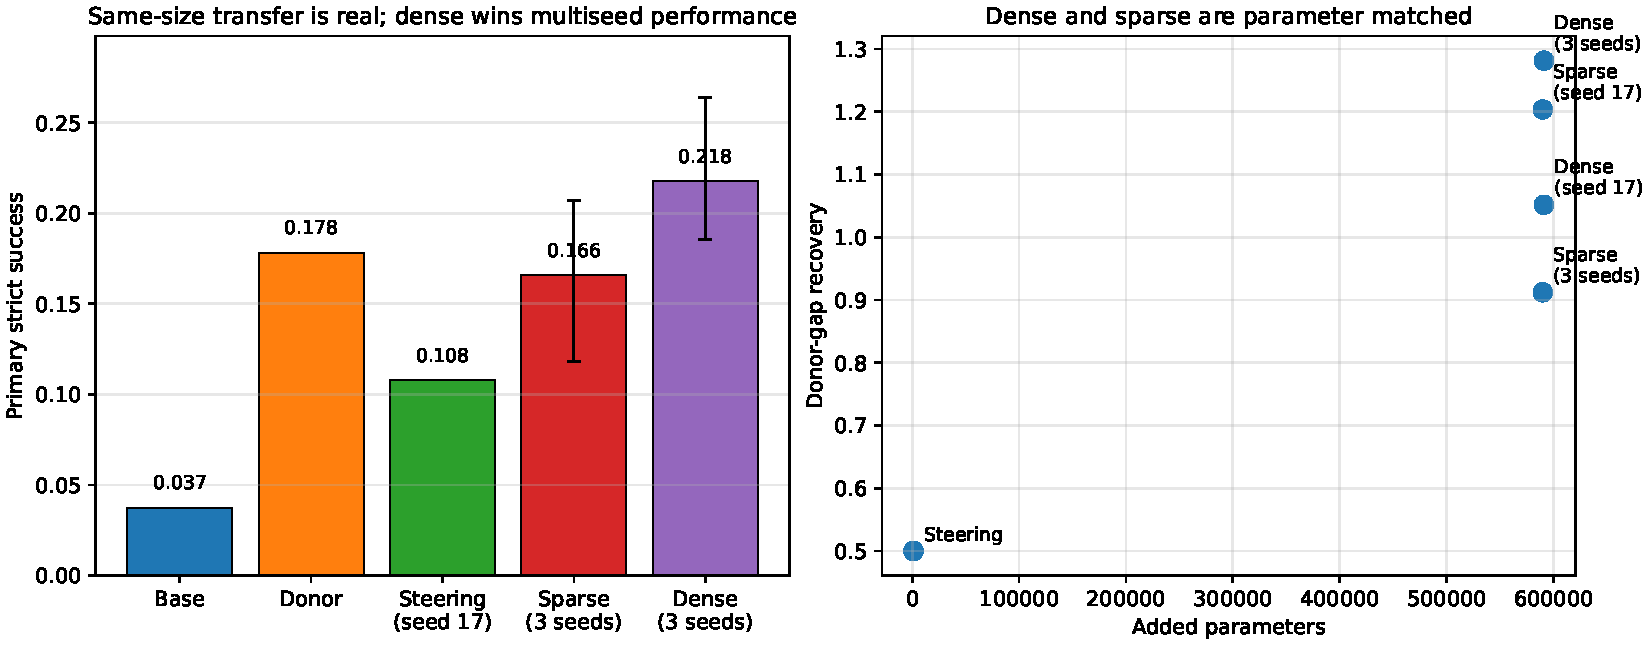
\includegraphics[width=0.98\textwidth]{figures/overview_tradeoff.pdf}
  \caption{Overview of the same-size transfer result. \textbf{Left:} the donor gap is real, sparse same-size transfer is real, and dense wins the final multiseed comparison. Error bars show 95\% bootstrap intervals for the multiseed means. \textbf{Right:} sparse and dense are effectively parameter matched, while steering is much cheaper and much weaker.}
  \label{fig:overview}
\end{figure*}

\subsection{Where the gains come from}
The slice breakdown in \Cref{fig:slices} clarifies why we avoid a broad semantic-transfer claim. SchemaShift strict success is essentially unchanged from the base for the sparse, dense, and steering interventions: all three remain at $0.0016$ on that slice, whereas the donor reaches $0.5344$. The same-size interventions therefore do \emph{not} reconstruct the donor's exact schema-shift semantics.

Instead, most of the primary-metric gain comes from NoCall behavior. On the unsupported-intent slice, sparse rises from $0.0406$ to $0.4953$, and dense rises to $0.4078$. On the missing-tool slice, base starts at $0.0703$, sparse reaches $0.1234$, and dense reaches $0.1469$. Semantic scores also improve over base, but the strongest movement remains concentrated in NoCall rather than renamed-schema exactness. The right conclusion is therefore not ``clean semantic transfer,'' but ``real structured-behavior transfer under a locked primary metric, with the strongest gains in abstention-like behavior.''

\begin{figure}[t]
  \centering
  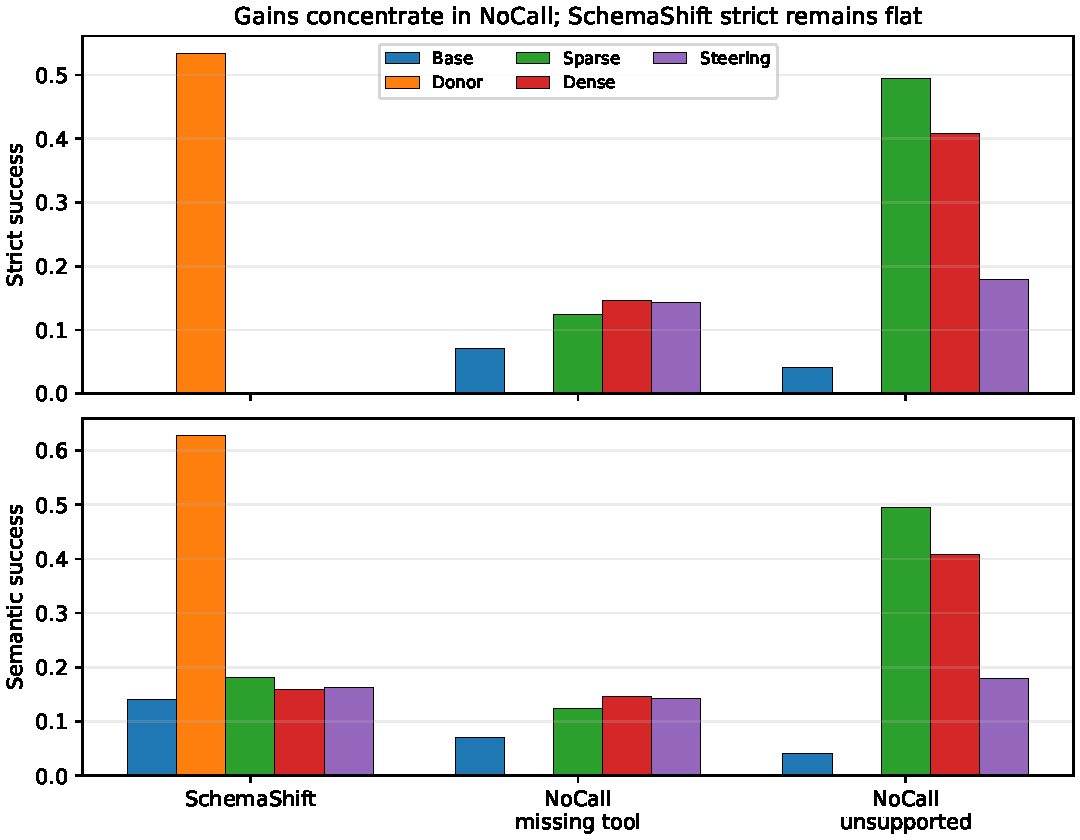
\includegraphics[width=\columnwidth]{figures/slice_breakdown.pdf}
  \caption{Per-slice strict and semantic success on the primary stress slices. The same-size interventions leave SchemaShift strict success at the base level but improve NoCall behavior substantially, especially on unsupported requests.}
  \label{fig:slices}
\end{figure}

\section{Localization analysis and controls}
The sparse intervention remains scientifically interesting because it exposes structure that the dense result alone would hide. \Cref{tab:localization} shows that a locked one-feature subset retains $47.1\%$ of the full sparse gain, with $0.1172$ strict success and no measured control drop on the frozen control suite. That one-feature subset also beats random one-feature controls, whose mean strict success is only $0.0566$; the best random one-feature control reaches $0.0833$.

This does not identify a unique circuit. The retained-gain fraction falls well short of the stronger $\ge 80\%$ bar that would justify a sharper sufficiency claim. But it does show that the sparse effect is not arbitrary. There is real localization structure in the selected sparse module, and that structure survives pruning and random-subset controls.

\begin{table}[t]
\centering
\caption{Pruning analysis for the sparse same-size intervention. The selected one-feature subset retains nearly half of the full sparse gain and clearly outperforms random one-feature controls, but it does not justify a uniqueness claim.}
\label{tab:localization}
\small

\begingroup
\hfuzz=6pt
\resizebox{\columnwidth}{!}{%
\begin{tabular}{@{}lS[table-format=3.0]S[table-format=1.4]S[table-format=1.4]S[table-format=1.4]@{}}
\toprule
System & {Features} & {Strict} & {Retained gain} & {Control drop} \\
\midrule
Full sparse module & 256 & 0.2068 & 1.0000 & -0.0141 \\
Selected subset & 1 & 0.1172 & 0.4708 & 0.0000 \\
Random 1-feature mean & 1 & 0.0566 & 0.1131 & -0.0008 \\
\bottomrule
\end{tabular}%
}
\endgroup

\end{table}

A second useful contrast comes from the shortcut baselines. One-vector steering is clearly weaker than either learned module. Dense and sparse, however, fail differently. On the discovery seed, sparse reduces parsing failures more aggressively than dense (rate $0.0479$ vs. $0.0880$), while dense makes fewer wrong-argument-key errors ($0.1490$ vs. $0.2063$). In other words, sparse appears to buy a crisper structural intervention, while dense buys more of the exact task behavior. That is the performance--localization tradeoff emphasized by the full set of results.

\section{Error analysis, robustness, and limitations}
The control-suite story is numerically reassuring but not decisive. Sparse multiseed control drop is $-0.0057$, and dense multiseed control drop is $-0.0109$. Both are small, and both stay within the predeclared tolerance. Sparse therefore has a slight numerical edge on collateral damage, but not a strong enough edge to support a broader narrowness claim.

The main robustness limitation is semantic scope. Our strongest improvements do not show up as renamed-schema exactness. Instead they concentrate in NoCall behavior, especially unsupported-intent abstention. This is still useful---hallucinated tool calls are a real failure mode in function-calling systems---but it is not the same thing as robust schema-grounded argument transfer. We therefore state the semantic claim narrowly and report strict and semantic metrics side by side.

The study is also limited by design. It is same-size only, within-family only, single-turn only, and V24-only. We do not claim cross-scale transfer, data efficiency relative to recipient tuning, universal model editing, or uniquely identified sparse circuits. The goal is not to solve all of capability transfer; it is to provide a clean same-size transfer result and show that raw performance and mechanistic compactness separate even in a tightly controlled setting.

\section{Conclusion}
We studied same-size capability transfer under a locked deterministic function-calling setup and found a real performance--localization tradeoff. The donor gap is real. A sparse same-size module can transfer meaningful structured behavior into the untuned base model, survives multiseed confirmation, beats steering, and retains a non-random localization signal under pruning. But the best-performing same-size mechanism in this study is not maximally sparse: a dense parameter-matched shortcut recovers more raw task performance on the final matched multiseed comparison.

That result is informative in its own right. It says that constructive transfer is possible without full retraining, but also that the most localized mechanism need not be the most performant one. In this deterministic function-calling setting, dense modules recover more behavior, sparse modules reveal more structure, and the two objectives do not collapse into a single optimum.

\bibliographystyle{plainnat}
\bibliography{references}

\appendix
\section{Additional setup details}
The same-size path uses a locked prompt contract, a fixed JSON output schema, and frozen manifests. Discovery uses one seed for candidate selection and gain calibration; final sparse and dense comparisons use three seeds on the same frozen manifests. The primary metric is evaluated on 640 SchemaShift examples, 640 NoCall-MissingTool examples, and 640 NoCall-Unsupported examples. Strict scoring requires exactly one valid JSON object with the correct normalized content. Semantic scoring recovers the first valid object even if extra text follows.

\section{Expanded slice metrics}
\begin{table}[H]
\centering
\caption{Strict and semantic results on the primary slices. These numbers explain why the paper avoids a broad semantic-transfer claim: aggregate gains do not come from SchemaShift strict success.}
\label{tab:appendix-slices}
\small

\begin{tabular}{llSS}
\toprule
System & Slice & {Strict} & {Semantic} \\
\midrule
Base & SchemaShift & 0.0016 & 0.1406 \\
Base & NoCall missing tool & 0.0703 & 0.0703 \\
Base & NoCall unsupported & 0.0406 & 0.0406 \\
\addlinespace
Donor & SchemaShift & 0.5344 & 0.6281 \\
Donor & NoCall missing tool & 0.0000 & 0.0000 \\
Donor & NoCall unsupported & 0.0000 & 0.0000 \\
\addlinespace
Sparse (seed 17) & SchemaShift & 0.0016 & 0.1813 \\
Sparse (seed 17) & NoCall missing tool & 0.1234 & 0.1234 \\
Sparse (seed 17) & NoCall unsupported & 0.4953 & 0.4953 \\
\addlinespace
Dense (seed 17) & SchemaShift & 0.0016 & 0.1594 \\
Dense (seed 17) & NoCall missing tool & 0.1469 & 0.1469 \\
Dense (seed 17) & NoCall unsupported & 0.4078 & 0.4078 \\
\addlinespace
Steering (seed 17) & SchemaShift & 0.0016 & 0.1625 \\
Steering (seed 17) & NoCall missing tool & 0.1422 & 0.1422 \\
Steering (seed 17) & NoCall unsupported & 0.1797 & 0.1797 \\
\bottomrule
\end{tabular}

\end{table}

\section{Error categories}
\begin{table}[H]
\centering
\caption{Primary-slice error profile for the base model, the sparse discovery-seed checkpoint, and the dense discovery-seed checkpoint. Sparse dramatically reduces parsing failures but does not dominate dense on argument-key accuracy.}
\label{tab:appendix-errors}
\small

\begin{tabular}{lSSS}
\toprule
Error category & {Base} & {Sparse (seed 17)} & {Dense (seed 17)} \\
\midrule
Parsing failure & 0.2036 & 0.0479 & 0.0880 \\
Wrong call vs. \texttt{NO\_TOOL} & 0.4531 & 0.4255 & 0.4286 \\
Wrong argument key & 0.0911 & 0.2063 & 0.1490 \\
Wrong tool & 0.1104 & 0.0521 & 0.0792 \\
Strict success & 0.0375 & 0.2068 & 0.1854 \\
\bottomrule
\end{tabular}

\end{table}

\begin{figure}[H]
  \centering
  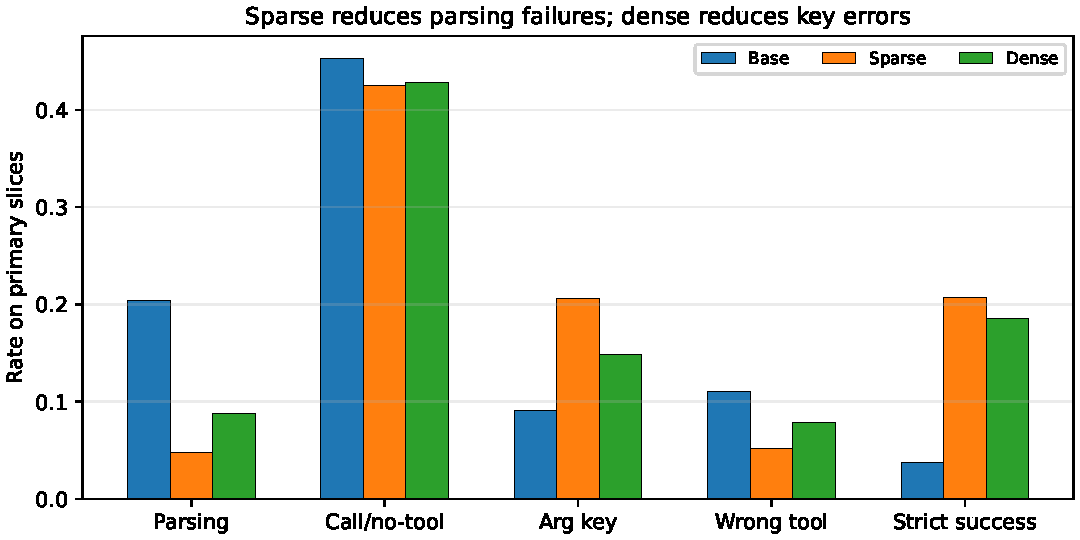
\includegraphics[width=\columnwidth]{figures/error_profile.pdf}
  \caption{Error-category view of the discovery-seed sparse and dense checkpoints. The sparse checkpoint is structurally cleaner in some categories, especially parsing, but not uniformly better.}
  \label{fig:error-profile}
\end{figure}

\section{Calibration sensitivity and localization}
\begin{figure}[H]
  \centering
  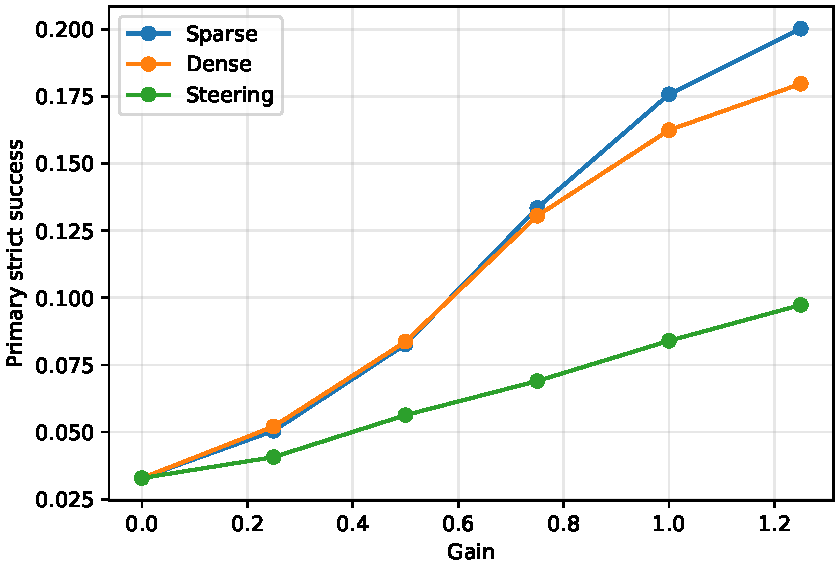
\includegraphics[width=0.9\columnwidth]{figures/calibration_sensitivity.pdf}
  \caption{Primary strict success as a function of gain on the locked calibration sweep. Sparse and dense both improve smoothly with gain, while steering remains substantially weaker throughout the sweep.}
  \label{fig:calib}
\end{figure}

\begin{figure}[H]
  \centering
  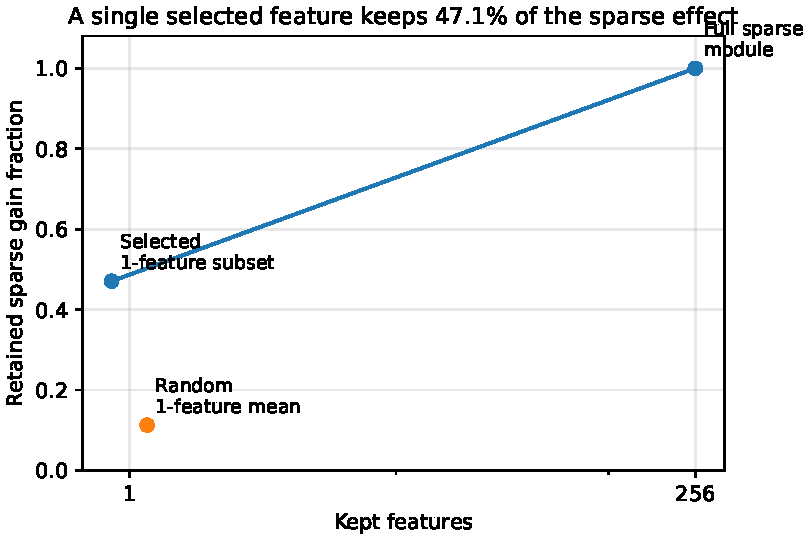
\includegraphics[width=0.8\columnwidth]{figures/localization_retained_gain.pdf}
  \caption{Retained sparse gain versus kept features. A single selected feature keeps 47.1\% of the full sparse effect, well above the random one-feature mean, but far below a uniqueness-style sufficiency bar.}
  \label{fig:retained}
\end{figure}

\section{Qualitative examples}
\begin{table}[H]
\centering
\caption{Representative qualitative patterns from the saved appendix examples. We summarize the patterns rather than reproducing raw outputs verbatim because many saved generations contain long parser-noise tails that are not informative in print.}
\label{tab:qualitative}
\small

\begin{tabularx}{\textwidth}{l l X}
\toprule
Case & Winner & Summary \\
\midrule
Unsupported request & Sparse over dense & On unsupported NoCall prompts, sparse often returned a single \texttt{NO\_TOOL} object where dense emitted extra fenced JSON or an unnecessary tool call. \\
Missing-tool request & Sparse over base & When the requested action was unavailable, sparse more often abstained with \texttt{NO\_TOOL} instead of forcing a tool call. \\
Surface-form robustness & Dense over sparse & Dense more often preserved argument keys correctly when a call was appropriate, while sparse more often failed on argument-key exactness. \\
Control suite & Tie / sparse edge & Sparse and steering produced no recorded control-damage examples in the saved appendix bundle; dense produced one capitalization-only deviation. \\
\bottomrule
\end{tabularx}

\end{table}

\end{document}
